%!TEX root =../quadrotorbook.tex
\chapter{Multirotor Equations of Motion}
\label{chap:multirotor}

Author: Tim McLain, RWB

\section{Equations of Motion}
Let $\mathcal{F}_i$ denote an earth-fixed inertial reference frame with unit vectors $(\mathbf{i}_i,\mathbf{j}_i,\mathbf{k}_i)$ aligned with the north, east, and down directions. Let $\mathcal{F}_b$ denote a reference frame that is fixed with respect to the multirotor body having unit vectors $(\mathbf{i}_b,\mathbf{j}_b,\mathbf{k}_b)$ aligned with the forward, right, and down directions in the body frame. The orientation of the multirotor with respect to the inertial reference frame can be expressed by the rotation matrix $R_b^i \in \mathit{SO}(3)$ which can be expressed as\cite{BeardMcLain12}
\begin{equation}
R_b^i = 
\begin{pmatrix} c_{\theta} c_{\psi} & s_{\phi} s_{\theta} c_{\psi} - c_{\phi} s_{\psi}
& c_{\phi} s_{\theta} c_{\psi} + s_{\phi} s_{\psi} \\
c_{\theta} s_{\psi} &  s_{\phi} s_{\theta} s_{\psi} + c_{\phi} c_{\psi}
  & c_{\phi} s_{\theta} s_{\psi} - s_{\phi} c_{\psi}  \\
-s_{\theta} & s_{\phi} c_{\theta} & c_{\phi} c_{\theta}
\end{pmatrix},
\label{eq:eom_rot_1}
\end{equation}
where we have used the notation $c_x\defeq\cos x$ and $s_x\defeq \sin x$. The angles $(\phi,\theta,\psi)$ are the roll, pitch, and yaw Euler angles. The rotation matrix in equation~\eqref{eq:eom_rot_1} corresponds to the yaw-pitch-roll (3-2-1) rotation sequence.

We can represent the rigid-body dynamics of the multirotor with the equations of motion
\begin{align*}
	\dot{\mathbf{p}}_{b/i}^i &= \mathbf{v}_{b/i}^i \\
	\dot{\mathbf{v}}_{b/i}^i &= g \kbf_i^i + \frac{1}{m} R_b^i \mathbf{F}^b \\
	\dot{R}_b^i &= R_b^i \ss{\omegabf_{b/i}^b} \\
	J\dot{\omegabf}_{b/i}^b &= -\omegabf_{b/i}^b \times (\Jbf\omegabf_{b/i}^b) + \taubf^b.
\end{align*}
%
In these equations, $m$ denotes the mass of the multirotor and $\Jbf$ is the inertia matrix of the multirotor with respect to the body-frame axes. The vectors $\Fbf^b$ and $\taubf^b$ define the aerodynamic forces and moments experienced by the multirotor and are expressed in the body frame. The vectors $v_{b/i}^i$, $\omegabf_{b/i}^i$, and $p_{b/i}^i$ are the velocity, angular velocity, and position of the multirotor with respect to the inertial reference frame as expressed in the inertial frame, while the variable $g$ denotes the gravitational constant. The notation $\ss{\omegabf}$ represents the skew-symmetric matrix operator formed from the vector $\omegabf$ so that $\ss{\omegabf} \vbf = \omegabf \cross \vbf$ for the vector cross product $\cross$ and any vector $\vbf \in \mathbb{R}^3$.



%%%%%%%%%%%%%%%%% BEGIN OMIT
%
% This stuff is potentially useful. Just taking it out while we get main ideas in place
%
\OMIT{
In this chapter,  we derive expressions for the kinematics and the
dynamics of a rigid body.  While the expressions derived in this
chapter are general to any rigid body, we will use notation and
coordinate frames that are common in the aeronautics literature. In 
Section~\ref{sec:eom-state-variables}, we define the
notation that will be used for the state variables of a quadrotor.
In Section~\ref{sec:eom-kinematics} we derive expressions for
the kinematic equations of motion, and in Section~\ref{sec:eom-dynamics} we derive the
dynamic equations of motion from Newton's 2nd law.

\twmcomment{Later sections to introduce EOM using quaternions?}

\section{State Variables}
\label{sec:eom-state-variables}

\twmcomment{What is the generic name that we will use for the aircraft? Quadrotor doesn't seem right since we want to generalize to $N$ rotors. Multirotor seems fine, but it is a little long. What will our abbreviation be? MR? QR? MRA (for multirotor aircraft)? I think we should figure out what the mainstream folks are doing.}

State variables describe the energy state of the quadrotor as it flies about and include linear and angular positions, as well as linear and angular velocities. These state variables and their derivatives with respect to time represent the dynamic behavior of the quadrotor and are related to one another by ordinary differential equations that we call the equations of motion. A standard set of state variables for the quadrotor can be seen in table~\ref{tab:eom-state-varibles}. Some of the state variables are derived with respect to inertial reference frames, while others are derived with respect to reference frames fixed in the body of the quadrotor. We first introduce state variables and equations of motion that use Euler angles to represent the attitude of the quadrotor. In later sections we will express the attitude in terms of a quaternion representation along with the corresponding changes to the equations of motion..

The position of the quadrotor is represented with respect to a fixed (inertial) location on the earth using a north-east-down reference frame with the variables ($p_n$, $p_e$, $p_d$) as the position states. The attitude, or angular orientation, of the quadrotor is represented by the Euler angles ($\phi$, $\theta$, $\psi$), which are defined as described in section~\ref{sec:rotation_matrices}. The translational velocity of the quadrotor is represented by the variables ($u$, $v$, $w$), which are the components of the velocity vector in the directions of the body-frame ($\mathbf{i}^b$, $\mathbf{j}^b$, $\mathbf{k}^b$) axes of the quadrotor. The angular velocity of the quadrotor is represented by the variables ($p$, $q$, $r$), which are the components of the angular rates along these same body-frame axes. These state variables are depicted schematically in figure~\ref{fig:eom-state-variables}.
%
\begin{table}
\centering
\caption{State variables for MAV equations of motion.}
\label{tab:eom-state-variables}
\vspace{0.07in}
\begin{tabular}{|c|l|}
\hline
Name & Description \\
\hline \hline
$p_n$ & Inertial north position of quadrotor along $\mathbf{i}^i$ in $\mathcal{F}^i$.\\  \hline
$p_e$ & Inertial east position of quadrotor along $\mathbf{j}^i$ in $\mathcal{F}^i$.\\  \hline
$p_d$ & Inertial down position (negative of altitude) of quadrotor along $\mathbf{k}^i$ in $\mathcal{F}^i$.\\  \hline
$u$ & Body-frame velocity measured along $\mathbf{i}^b$ in $\mathcal{F}^b$.\\  \hline
$v$ & Body-frame velocity measured along $\mathbf{j}^b$ in $\mathcal{F}^b$.\\  \hline
$w$ & Body-frame velocity measured along $\mathbf{k}^b$ in $\mathcal{F}^b$.\\  \hline
$\phi$ & Roll angle defined with respect to $\mathcal{F}^{v2}$.\\  \hline
$\theta$ & Pitch angle defined with respect to $\mathcal{F}^{v1}$.\\  \hline
$\psi$ & Heading (yaw) angle defined with respect to $\mathcal{F}^v$. \\  \hline
$p$ & Roll rate measured along $\mathbf{i}^b$ in $\mathcal{F}^b$. \\  \hline
$q$ & Pitch rate measured along $\mathbf{j}^b$ in $\mathcal{F}^b$. \\  \hline
$r$ & Yaw rate measured along $\mathbf{k}^b$ in $\mathcal{F}^b$. \\
\hline
\end{tabular}
\end{table} \index{State Variables}
%
The body-frame axes of the quadrotor ($\mathbf{i}^b$, $\mathbf{j}^b$, $\mathbf{k}^b$) are commonly referred to as the roll, pitch, and yaw axes of the quadrotor respectively. The roll, pitch, and yaw rates ($p$, $q$, $r$) are measured about these axes. As explained in section~\ref{sec:frames-quadrotor-frames}, the Euler angles describing the yaw displacement $\psi$ and pitch displacement $\theta$ of the aircraft are defined by rotations about the $\mathbf{k}^{v}$ = $\mathbf{k}^{v1}$ and $\mathbf{j}^{v1}$ = $\mathbf{j}^{v2}$ axes that are not aligned with the body frame $\mathcal{F}^b$. Because of this, $\psi$ and $\theta$ cannot be expressed simply as rotations about the yaw and pitch axes of the aircraft. Furthermore, the pitch and yaw rates, $q$ and $r$, are not equivalent to the time derivatives of the pitch and yaw angles, $\theta$ and $\psi$. 
%
\begin{figure}[hhhhtb]
\begin{center}
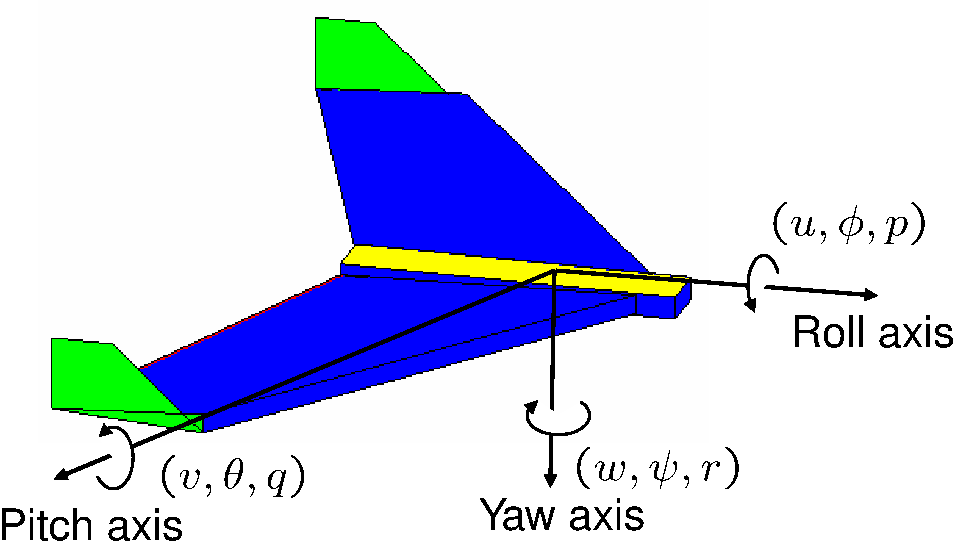
\includegraphics[width=3.5in]{chap3_multirotor/figures/kin-axis-definition}
\end{center}
\caption{Graphical definition of state variables.} \label{fig:eom-state-variables}
\end{figure}

\section{Kinematic Equations of Motion}
As we set out to derive equations of motion for the quadrotor, our goal is come up with relationships expressing derivatives of state variables in terms of state variables and inputs to the system. The kinematic equations describing the motion of the quadrotor, will involve relationships between derivatives of the position states and the velocity states without any consideration for the inputs to the system. In the sections that follow, we will first consider the translational kinematics, followed by the rotational kinematics.

\subsection{Translational Kinematics}
The translational kinematic equations of motion represent the relationship between the time derivatives of the position state variables ($\dot{p}_n$, $\dot{p}_e$, $\dot{p}_d$) that are defined with respect to a fixed inertial reference frame and the velocity state variables ($u$, $v$, $w$) that are defined with respect to the body frame of the quadrotor. Taking advantage of the rotational transformation between the body and vehicle (inertial) frame derived in equation~\eqref{eq:frames-Rvb}, the relationship between the translational positions and velocities is given by
\begin{equation*}
\frac{d}{dt} \begin{pmatrix} p_n \\ p_e \\ p_d \end{pmatrix} =
\mathcal{R}_{b}^{v} \begin{pmatrix} u \\ v \\ w \end{pmatrix}
= (\mathcal{R}_{v}^{b})^{\top} \begin{pmatrix} u \\ v \\ w \end{pmatrix} ,
\end{equation*}
which leads to
\begin{equation}
\begin{pmatrix} \dot{p}_n \\ \dot{p}_e \\ \dot{p}_d \end{pmatrix} = \begin{pmatrix} c_{\theta} c_{\psi} & s_{\phi} s_{\theta} c_{\psi} - c_{\phi} s_{\psi}
& c_{\phi} s_{\theta} c_{\psi} + s_{\phi} s_{\psi} \\
c_{\theta} s_{\psi} &  s_{\phi} s_{\theta} s_{\psi} + c_{\phi} c_{\psi}
  & c_{\phi} s_{\theta} s_{\psi} - s_{\phi} c_{\psi}  \\
-s_{\theta} & s_{\phi} c_{\theta} & c_{\phi} c_{\theta}
\end{pmatrix}
\begin{pmatrix} u \\ v \\ w \end{pmatrix},
\label{eq:kin-trans-1}
\end{equation}
where we have used the notation $c_x\defeq\cos x$ and $s_x\defeq \sin x$. These equations represent three of the 12 state equations that we will define.

\subsection{Rotational Kinematics} 
The rotational kinematic equations of motion relate the time derivatives of the Euler angles ($\dot{\phi}$, $\dot{\theta}$, $\dot{\psi}$) and the body-frame angular rates ($p$, $q$, $r$). While the angular motion represented by $\dot{\phi}$ can be thought of as a rotation about the body-frame $\mathbf{i}^b$ axis, the motions represented by $\dot{\theta}$ and $\dot{\psi}$ are not defined as rotations about unique body axes. Instead, they are defined in section~\ref{sec:rotation_matrices} as rotations about the intermediate axes $\mathbf{j}^{v2}$ and $\mathbf{k}^{v1}$ respectively. We can relate these Euler angle derivatives to the body-fixed angular rates by rotating the Euler angle derivatives into the body-fixed reference frame and summing them to give
\begin{align}
\begin{pmatrix} p \\ q \\ r \end{pmatrix} &=
\begin{pmatrix} \dot{\phi} \\ 0 \\ 0
\end{pmatrix}
+ \mathcal{R}_{v2}^{b}(\phi) \begin{pmatrix} 0 \\ \dot{\theta} \\
0 \end{pmatrix} + \mathcal{R}_{v2}^{b}(\phi) \mathcal{R}_{v1}^{v2}(\theta)
    \begin{pmatrix} 0 \\ 0 \\ \dot{\psi} \end{pmatrix}  \notag \\
&= \begin{pmatrix} \dot{\phi} \\ 0 \\ 0 \end{pmatrix}
+ \begin{pmatrix}
    1 & 0 & 0 \\
    0 & c_{\phi} & s_{\phi} \\
    0 & -s_{\phi} & c_{\phi}
  \end{pmatrix}
  \begin{pmatrix} 0 \\ \dot{\theta} \\ 0 \end{pmatrix}
+ \begin{pmatrix}
    1 & 0 & 0 \\
    0 & c_{\phi} & s_{\phi} \\
    0 & -s_{\phi} & c_{\phi}
  \end{pmatrix}
  \begin{pmatrix}
    c_{\theta} & 0 & -s_{\theta} \\
    0 & 1 & 0 \\
    s_{\theta} & 0 & c_{\theta}
  \end{pmatrix}
  \begin{pmatrix} 0 \\ 0 \\ \dot{\psi} \end{pmatrix}  \notag \\
&= \begin{pmatrix}
  1 & 0 & -s_{\theta} \\
  0 & c_{\phi} & s_{\phi} c_{\theta} \\
  0 & -s_{\phi} & c_{\phi} c_{\theta}
\end{pmatrix}
\begin{pmatrix} \dot{\phi} \\ \dot{\theta} \\ \dot{\psi} \end{pmatrix}.
\label{eq:kin-phithetapsidot-to-pqr}
\end{align}
Inverting this expression leads to the rotational kinematic equations of motion\index{Kinematics!Rotation}
\begin{equation} \label{eq:kin-rotational-kinematics}
\begin{pmatrix} \dot{\phi} \\ \dot{\theta} \\ \dot{\psi} \end{pmatrix}
= \begin{pmatrix}
  1 & \sin\phi\tan\theta & \cos\phi\tan\theta \\
  0 & \cos\phi & -\sin\phi \\
  0 & \sin\phi\sec\theta & \cos\phi\sec\theta
  \end{pmatrix}
  \begin{pmatrix} p \\ q \\ r \end{pmatrix} ,
\end{equation}
%
These equations express the derivatives of the three angular position states in terms of
the angular positions $\phi$ and $\theta$ and the body angular rates $p$, $q$, and $r$.

\twmcomment{I included the angular stuff for my own benefit. Once we have chapters 2 and 3 laid out, we can decide what goes where. I'd like to understand the new formulations of the EOM, so I will probably write about them to learn -- not trying to dictate what goes where.}

\twmcomment{START HERE!!!}

\section{Dynamic Equations of Motion}

- Do both translational and rotational dynamics

\subsection{Gravity Force}

}
%%%%%%%%%% END OMIT

%%%% Start here -- integrate induced drag into discussion

\subsection{Rotor Forces and Torques}
The aerodynamic forces and torques that enable the agile flight of a multirotor come from the dc-motor/propeller modules that we call the rotors. In hover, the rotors of a multirotor each provide a constant and equal thrust to overcome the effects of gravity. The rotors of a multirotor are usually configured in counter-rotating pairs, one rotating clockwise and the other counter-clockwise, so that the motor torques acting on the multirotor cancel out  when in a non-rotating hover state. As the rotors rotate, the drag on the propellers produce a torque on the body of the aircraft opposite to the direction of rotation. Figure~\ref{fig:eom-octo-std-def} depicts an octocopter with equally spaced counter-rotating rotors as an example of how a multirotor can be configured.

% Give marginfigures a try
\begin{marginfigure}
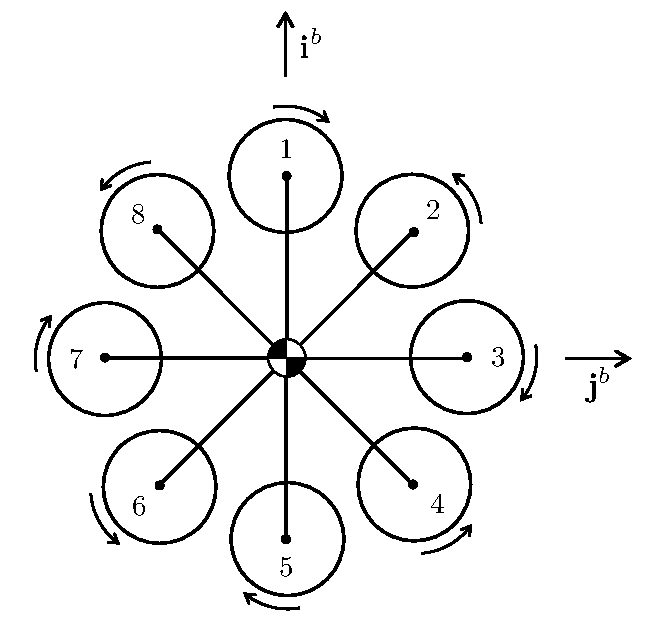
\includegraphics{chap3_multirotor/figures/eom-octo-std-def}
\caption{Octocopter example of a multirotor configuration.} 
\label{fig:eom-octo-std-def}
\end{marginfigure}
%

To accelerate the multirotor up or down, the speed of the rotors can be uniformly increased or decreased away from their nominal speed. To pitch up or down about the $\mathbf{j}_b$ axis, the speed differential between the fore and aft rotors can be sped up or slowed down. Similarly, to roll the aircraft right or left about the $\mathbf{i}_b$ axis the speed differential between the left and right rotors can be varied. To yaw the aircraft about the $\mathbf{k}_b$ axis, on the other hand, the speed differential between the clockwise-rotating props and counter-clockwise-rotating props is varied.

In modeling the aerodynamic forces and torques acting on the multirotor, we will consider thrust force $F_\text{thrust}$, the drag force $F_\text{drag}$, and the torque produced by the rotors. In this section, we will develop the relationship between the thrust force $F_{\text{thrust}}$, the roll, pitch, and yaw torques ($\tau_x$, $\tau_y$, $\tau_z$) and the individual rotor angular speeds. For an $N$-rotor aircraft, these angular speeds will be given by ($\omega_1$, $\omega_2$, $\ldots$, $\omega_N$) and specified in radians per second. From propeller theory, the thrust and torque produced by a single rotor in hover can be modeled as
\begin{align}
	T_i &= C_T \frac{\rho D^4}{4\pi^2} \omega_i^2	\\
	Q_i &= C_Q \frac{\rho D^5}{4\pi^2} \omega_i^2,	
\end{align}
where $\rho$ is the density of air, $D$ is the propeller diameter, and $C_T$ and $C_Q$ are non-dimensional aerodynamic coefficients specific to the propeller. 




The total rotor thrust for the multirotor is given by
\begin{equation}
   F_{\text{thrust}} = \sum\limits_{i=1}^N T_i ,
\end{equation}
where $F_i$ is the thrust force produced by rotor $i$.

%The negative sign takes into account that the thrust force is up in the body frame of the aircraft, while we have defined $F_z$ as positive down in the body frame. 

To define the torques produced by the rotors, we need to define the configuration of each rotor relative to the center of mass of the aircraft and its direction of rotation. Figure~\ref{fig:eom-rotor-definition} highlights a single rotor $i$ for an arbitrary multirotor configuration. The variable $\varphi_i$ is the angle between the forward direction of the multirotor, defined by the unit vector $\mathbf{i}^b$, and the radial direction of the $i^{\mathit{th}}$ rotor. The variable $\ell_i$ represents the radial distance from the center of mass to the $i^{\mathit{th}}$ rotor. The variable $d_i$ indicates the direction of rotation for each rotor as
%
%
\begin{marginfigure}
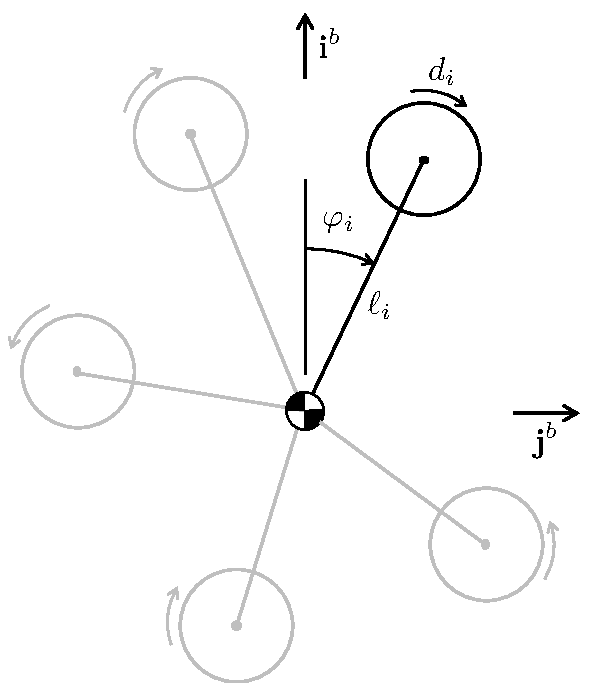
\includegraphics{chap3_multirotor/figures/eom-rotor-definition}
\caption{Definition of rotor configuration variables.} 
\label{fig:eom-rotor-definition}
\end{marginfigure}
%
%
\begin{equation}
   d_i = 
   \begin{cases}
      -1 	& \text{for CW rotation} \\
      +1 	& \text{for CCW rotation} .
   \end{cases}
\end{equation}
%
From the configuration geometry of Figure~\ref{fig:eom-rotor-definition}, the total roll torque about the $\mathbf{i}_b$ axis is given by
\begin{equation}
   \tau_x = - \sum\limits_{i=1}^N \left( \ell_i \sin \varphi_i \right) T_i .
\end{equation}
Similarly, the total pitch torque about the $\mathbf{j}_b$ axis can be calculated as
\begin{equation}
   \tau_y = \sum\limits_{i=1}^N \left( \ell_i \cos \varphi_i \right) T_i .
\end{equation}
Finally, the total yaw torque about the $\mathbf{k}_b$ axis, which depends on the direction of rotation of each rotor, is given by
\begin{equation}
   \tau_z = \sum\limits_{i=1}^N d_i Q_i .
\end{equation}
%
%
%\begin{marginfigure}
%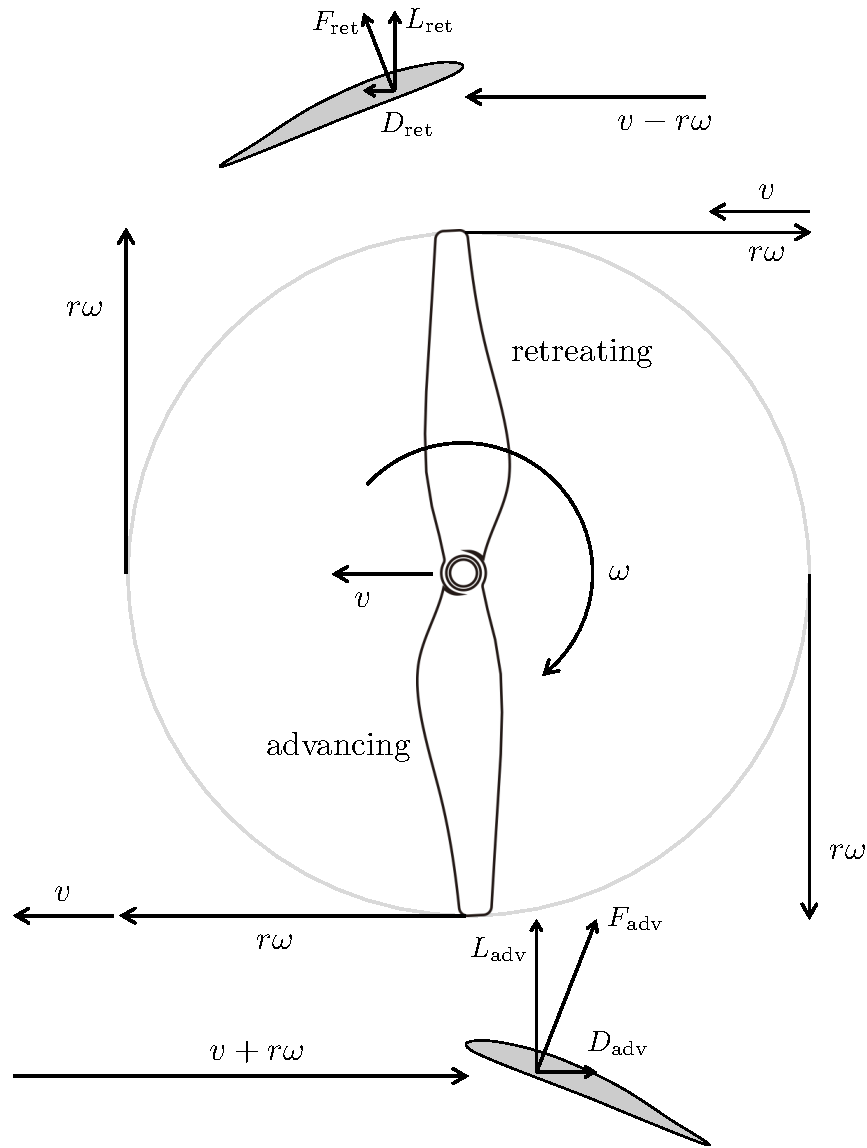
\includegraphics{chap3_multirotor/figures/eom-induced-drag}
%\caption{Induced rotor drag concept.} 
%\label{fig:eom-induced-drag}
%\end{marginfigure}
%
%

As with any lifting surface, induced drag forces are generated from the lift forces created by the rotating propellers. The direction of the drag force on a propeller blade at any instant is in the direction opposite of the velocity of the blade tip. Since the blade tip is moving much faster than the airspeed of the multirotor motion. When the blade is advancing into the oncoming apparent wind generated by the combination of multirotor motion and the wind, the induced drag is higher than when the blade is in the retreating portion of its circular motion and moving with the apparent wind. The net effect is that each of the rotors on the aircraft creates an induced drag force that is in the plane of the rotor and proportional to the projection of the lift force onto the plane of the rotor in magnitude and directed opposite to the airspeed vector. 
%
\begin{figure}[hhhhtb]
\begin{center}
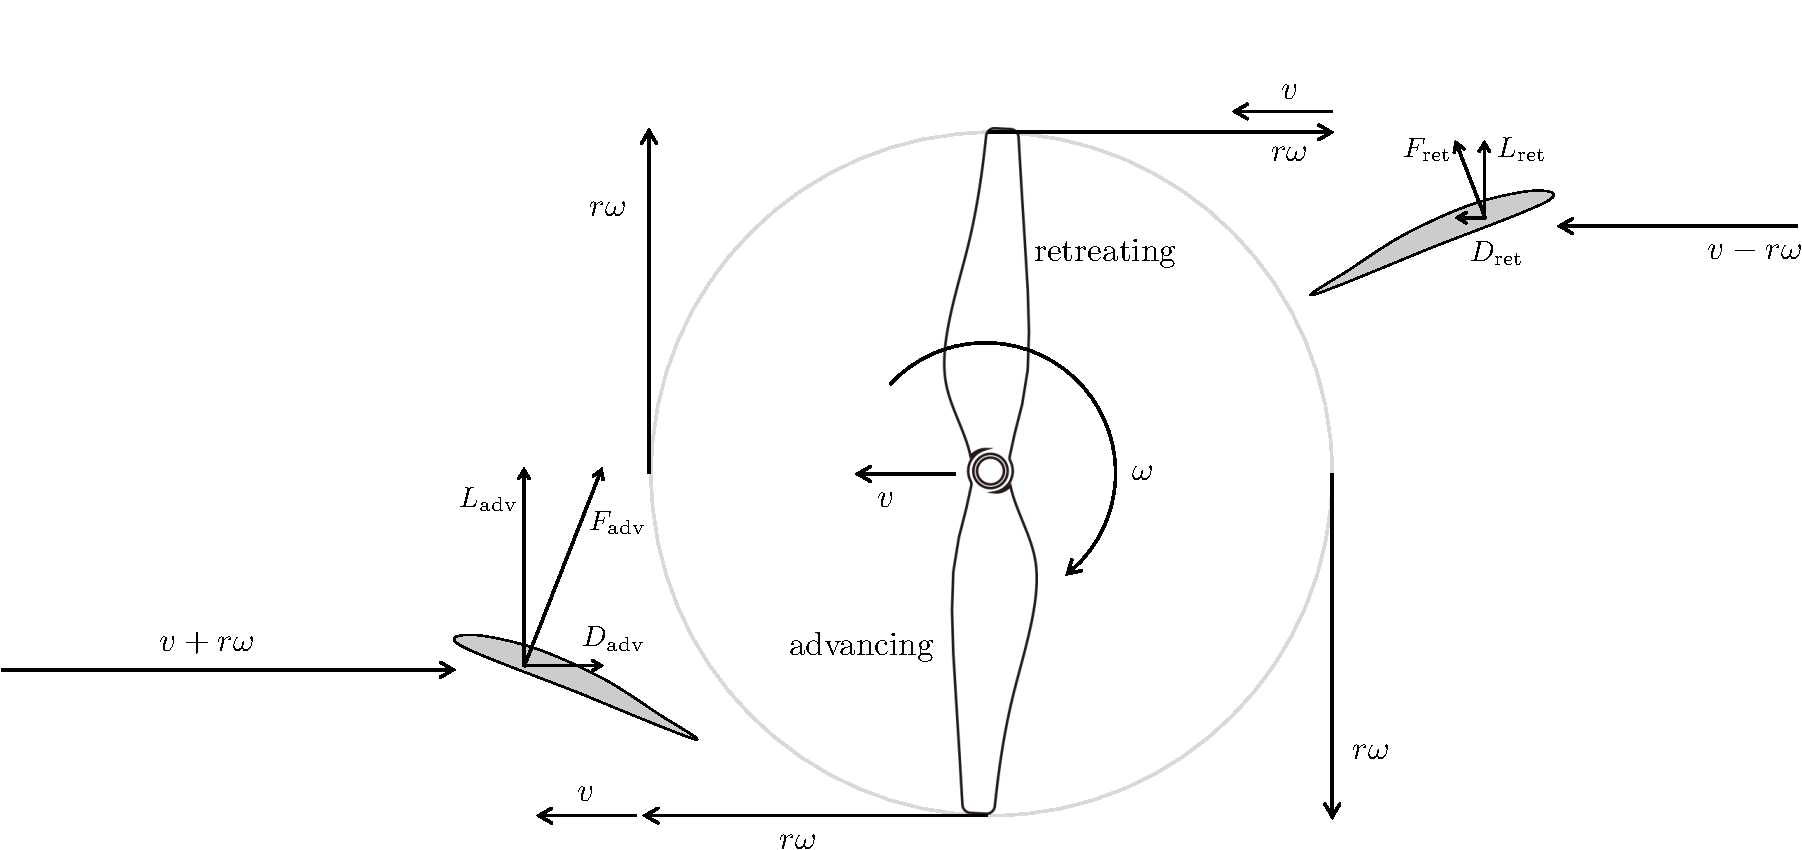
\includegraphics[width=6.5in]{chap3_multirotor/figures/eom-induced-drag2}
\end{center}
\caption{Induced drag.} \label{fig:eom-induced-drag}
\end{figure}
%
%
The drag force is also proportional to the component of the airspeed in the rotor plane.\cite{MahonyKC12} Accordingly, the drag force can be represented as 
\begin{align*}
	\Fbf_\text{drag}^b &\approx - F_\text{thrust} C_d \; \text{diag}(1,1,0) \vbf_{b/i}^b \\
	&= \begin{pmatrix} F_\text{thrust}C_d & 0 & 0 \\ 0 & F_\text{thrust}C_d & 0 \\ 0 & 0 & 0 \end{pmatrix}\vbf_{b/i}^b.
\end{align*}
Since the thrust force is approximately equal to $mg$, the weight of the aircraft, we can define
\[
D = \begin{pmatrix} gC_d & 0 & 0 \\ 0 & gC_d & 0 \\ 0 & 0 & 0 \end{pmatrix}
\]
and write induced drag in the body frame as
\begin{align*}
	\Fbf_\text{drag}^b &\approx mD R_b^{i\top} \vbf_{b/i}^i.	\label{eq:induced drag}
\end{align*}
In the following we write the thrust force as
\[
F_{\text{thrust}} = mT,
\]
where $T$ is the throttle setting.  
%
Therefore, the total aerodynamic force in the body frame is approximated as
\begin{align}
	\Fbf^b &\approx - mT \kbf_b^b + mD R_b^{i\top} \vbf_{b/i}^i.
\end{align}
In the inertial frame, the aerodynamic force is \sidenote{Recall that $\kbf_b^b = \ebf_3 = (0, 0, 1)^\top$}.
\begin{align}
	\Fbf^i &\approx - m T \ebf_3 + m R D R_b^{i\top} \vbf_{b/i}^i.
\end{align}


\section{Multirotor Mass Properties}
The mass properties of multirotors of particular interest to us are its mass $m$, center of mass location, and its inertia matrix $\Jbf$. The mass of a multirotor is distributed over the aircraft and the inertia matrix models how the mass is distributed and its effect on the rotational dynamics of the aircraft. Because the distribution of the mass of the aircraft is fixed in the body frame, $\Jbf$ is constant with respect to the body axes $(\ibf_b, \jbf_b, \kbf_b)$ and can be calculated as
\begin{align*}
\mathbf{J} &=
    \begin{pmatrix}
    \int (y^2 + z^2)\,dm & -\int xy\,dm         & -\int xz\,dm \\
    -\int xy\,dm         & \int (x^2 + z^2)\,dm &  -\int yz\,dm \\
    -\int xz\,dm         & -\int yz\,dm         & \int (x^2 + y^2)\,dm
    \end{pmatrix} \\
&\defeq
    \begin{pmatrix}
    J_{x}   & -J_{xy} & -J_{xz} \\
    -J_{xy} & J_{y}   & -J_{yz} \\
    -J_{xz} & -J_{yz} & J_{z}
    \end{pmatrix} .
\end{align*}

The diagonal terms of $\Jbf$ are called the moments of inertia and the off-diagonal terms are called the products of inertia. Multirotor aircraft tend to be symmetric in their shape and mass distribution and this results in significant simplification in the inertia matrix. In particular, if the aircraft is symmetric with respect to the $\ibf_b$-$\jbf$, $\ibf_b$-$\kbf$, and $\jbf_b$-$\kbf$ planes, then the products of inertia, $J_{xy}$, $J_{xz}$, and $J_{yz}=0$, are zero resulting in
\[
\mathbf{J} =
    \begin{pmatrix}
    J_{x}   & 0       & 0 \\
    0       & J_{y}   & 0 \\
    0 & 0       & J_{z}
    \end{pmatrix}.
\]
%
\begin{marginfigure}
	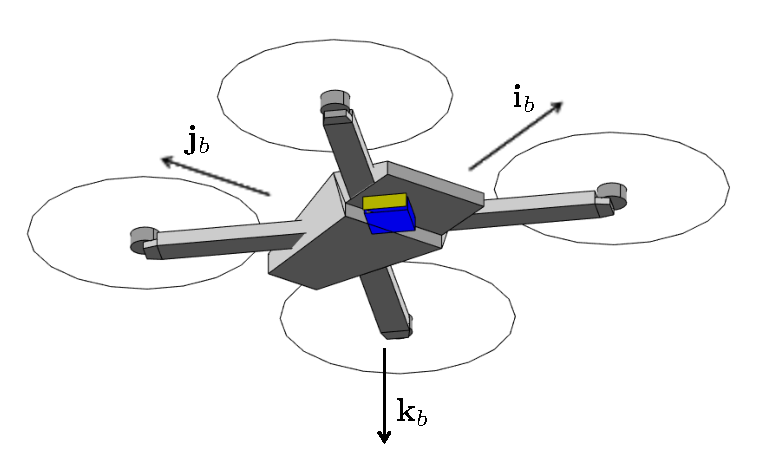
\includegraphics{chap3_multirotor/figures/eom-quad-axes}
	\caption{Quadrotor with body-frame axes that coincide at the center of mass.}
	\label{fig:eom-quad-axes}
\end{marginfigure}
%
Importantly, under these symmetry conditions, $\Jbf$ is easily inverted with its inverse expressed as
\begin{align*}
\mathbf{J}^{-1}
    &= \begin{pmatrix}
        \frac{1}{J_x} & 0 & 0 \\
        0 & \frac{1}{J_y} & 0 \\
        0 & 0 & \frac{1}{J_z}
       \end{pmatrix} .
\end{align*}

If a high-quality CAD model is available, the moments and products of inertia and the center of mass location can commonly be calculated numerically using the CAD software. Alternatively, moments of inertia and the center of mass location can be measured experimentally using equipment such as a bifilar pendulum. For simple geometries, the moments of inertia and center of mass can be calculated from moments of inertia of basic shapes and the parallel axis theorem. For example, the moments of inertia for the quadrotor shown in Figure~\ref{fig:eom-quad-axes} can be calculated by assuming that the quadrotor body is approximated by a cuboid with a specific length, width, mass, and uniform density. The rotor motors, arms, and propellers can be approximated as point masses located at the motor positions.

Summarizing, the equations of motion for the multirotor are given by
\begin{align}
	\dot{\pbf}_{b/i}^i &= \vbf_{b/i}^i \label{eq:eom_p} \\
	\dot{\vbf}_{b/i}^i &= g \ebf_3 - TR_b^i \ebf_3 + R_b^i D R_b^{i\top} \vbf_{b/i}^i  \label{eq:eom_v} \\
	\dot{R}_b^i &= R_b^i \ss{\omegabf_{b/i}^b} \label{eq:eom_R} \\
	J\dot{\omegabf}_{b/i}^b &= -\omegabf_{b/i}^b \times (J\omegabf_{b/i}^b) + \taubf^b. \label{eq:eom_omega}
\end{align}



%%%%%%%%%%%%%%%%%%%% Begin BIG omit
\OMIT{
%
%\begin{figure}[hhhhtb]
%\begin{center}
%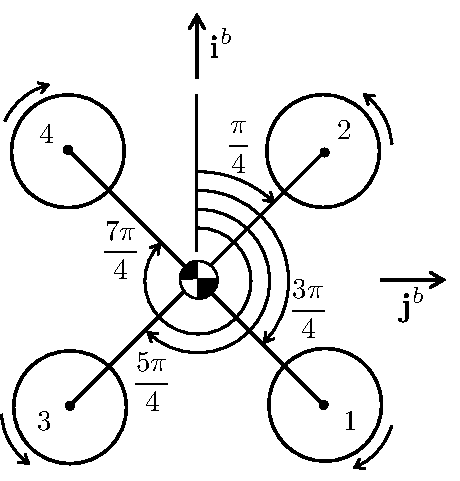
\includegraphics[width=3.0in]{chap3_multirotor/figures/eom-CF-quadX}
%\end{center}
%\caption{Definition of rotor variables for Cleanflight Quad X configuration.} \label{fig:eom-CF-quadX}
%\end{figure}
%

%
%\begin{figure}[hhhhtb]
%\begin{center}
%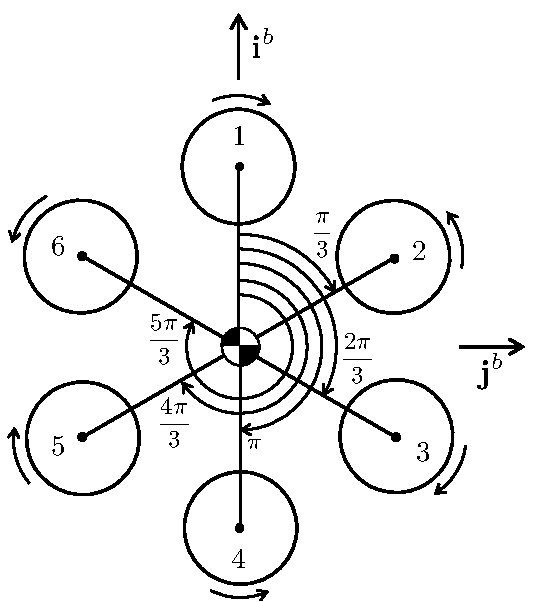
\includegraphics[width=3.0in]{chap3_multirotor/figures/eom-CF-hexa-plus}
%\end{center}
%\caption{Definition of rotor variables for Cleanflight Hexa Plus configuration.} \label{fig:eom-CF-hexa-plus}
%\end{figure}
%

%
%\begin{figure}[hhhhtb]
%\begin{center}
%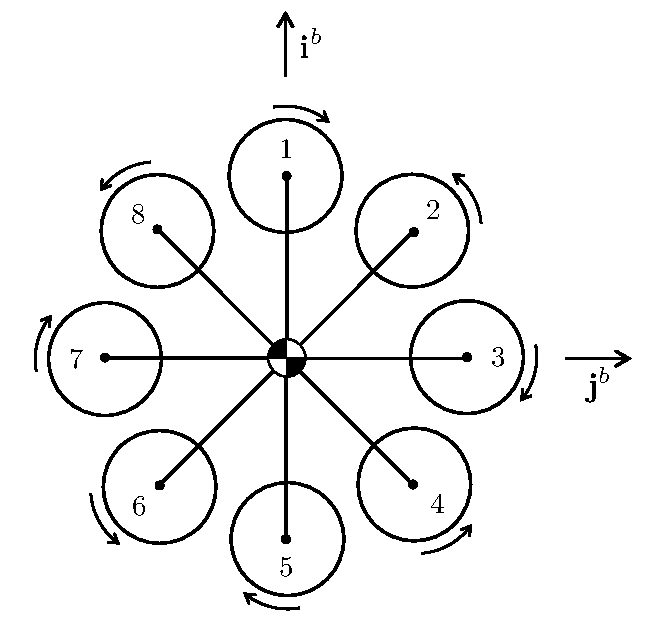
\includegraphics[width=3.5in]{chap3_multirotor/figures/eom-octo-std-def}
%\end{center}
%\caption{Recommended standard for rotor configuration variables.} \label{fig:eom-octo-std-def}
%\end{figure}
%


%- discuss the forces and moments due to different rotor configurations.   Make this part as general as possible to show how a variety of configurations can be handled.
%
%- Discussion of rotor drag term in translational dynamics
%
%- Rotor model (could get Andrew Ning to help out here)

\section{Body Frame Equations of Motion}

- Body relative equations of motion.  Provide some motivation for this model.

\section{Simplified Equations of Motion}

Show how certain assumptions lead to simplified equations of motion

- Euler angle models when roll and pitch angles are small

- equations of motion relative to a target, etc.


\section{Old stuff that might be useful}


%\chapter{Mathematical Preliminaries}
\section{Kinematics and Dynamics} \label{chap:kinematics}

In this chapter we derive the expressions for the kinematics and the
dynamics of a rigid body.  While the expressions derived in this
chapter are general to any rigid body, we will use notation and
coordinate frames that are typical in the aeronautics literature. In
particular, in Section~\ref{sec:kin-state-variables} we define the
notation that will be used for the state variables of a quadrotor.
In Section~\ref{sec:kin-kinematics} we derive the expressions for
the kinematics, and in Section~\ref{sec:kin-dynamics} we derive the
dynamics.



%%+++++++++++++++++++
\subsection{Quadrotor State Variables} %
\label{sec:kin-state-variables}

The state variables of the quadrotor are the following twelve
quantities
\begin{align*}
p_n &= \text{~the inertial (north) position of the quadrotor along $\hat{i}^i$ in $\mathcal{F}^i$,}\\
p_e &= \text{~the inertial (east) position of the quadrotor along $\hat{j}^i$ in $\mathcal{F}^i$,}\\
h &= \text{~the altitude of the aircraft measured along $-\hat{k}^i$ in $\mathcal{F}^i$,}\\
u &= \text{~the body frame velocity measured along $\hat{i}^b$ in $\mathcal{F}^b$,}\\
v &= \text{~the body frame velocity measured along $\hat{j}^b$ in $\mathcal{F}^b$,}\\
w &= \text{~the body frame velocity measured along $\hat{k}^b$ in $\mathcal{F}^b$,}\\
\phi &= \text{~the roll angle defined with respect to $\mathcal{F}^{v2}$,}\\
\theta &= \text{~the pitch angle defined with respect to $\mathcal{F}^{v1}$,}\\
\psi &= \text{~the yaw angle defined with respect to $\mathcal{F}^v$,} \\
p &= \text{~the roll rate measured along $\hat{i}^b$ in $\mathcal{F}^b$,}\\
q &= \text{~the pitch rate measured along $\hat{j}^b$ in $\mathcal{F}^b$,} \\
r &= \text{~the yaw rate measured along $\hat{k}^b$ in
$\mathcal{F}^b$.}
\end{align*}
The state variables are shown schematically in
Figure~\ref{fig:kin-axis-definition}.
%
\begin{figure}[hhhhtb]
\begin{center}
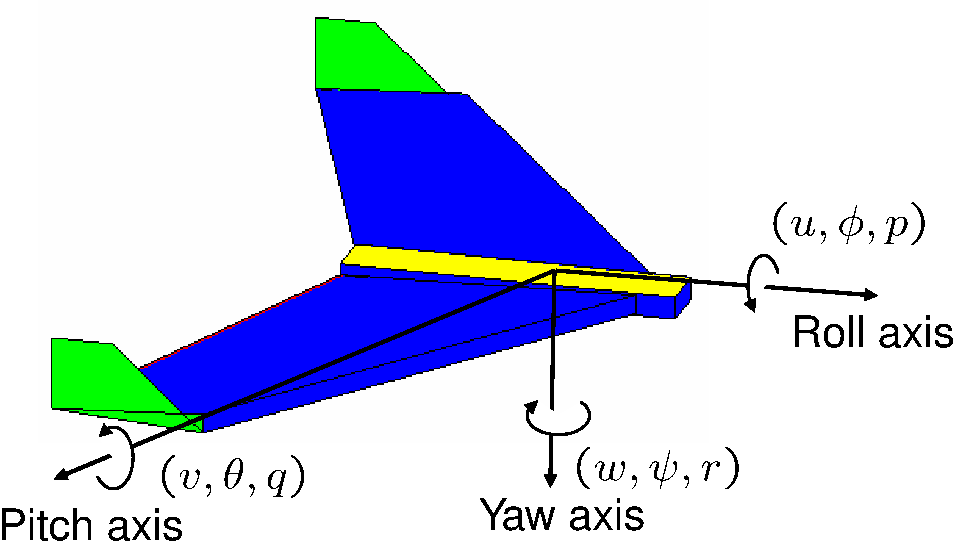
\includegraphics[width=3.0in]{chap3_multirotor/figures/kin-axis-definition}
\end{center}
\caption{Definition of Axes} \label{fig:kin-axis-definition}
\end{figure}
%
The position $(p_n, p_e, h)$ of the quadrotor is given in the
inertial frame, with positive $h$ defined along the negative $Z$
axis in the inertial frame.  The velocity $(u,v,w)$ and the angular
velocity $(p,q,r)$ of the quadrotor are given with respect to the
body frame.  The Euler angles (roll $\phi$, pitch $\theta$, and yaw
$\chi$) are given with respect to the vehicle 2-frame, the vehicle
1-frame, and the vehicle frame respectively.





%%+++++++++++++++++++
\subsection{Quadrotor Kinematics} %
\label{sec:kin-kinematics}

The state variables $p_n$, $p_e$, and $-h$ are inertial frame
quantities, whereas the velocities $u$, $v$, and $w$ are body frame
quantities. Therefore the relationship between position and
velocities is given by
\begin{align*}
\frac{d}{dt} \begin{pmatrix} p_n \\ p_e \\ -h \end{pmatrix} &=
R_{b}^{v} \begin{pmatrix} u \\ v \\ w \end{pmatrix} \\
&= (R_{v}^{b})^T \begin{pmatrix} u \\ v \\ w \end{pmatrix} \\
&= \begin{pmatrix} c\theta c\psi & s\phi s\theta c\psi - c\phi s\psi
& c\phi s\theta
c\psi + s\phi s\psi \\
c\theta s\psi &  s\phi s\theta s\psi + c\phi c\psi
  & c\phi s\theta s\psi - s\phi c\psi  \\
-s\theta & s\phi c\theta & c\phi c\theta
\end{pmatrix}
\begin{pmatrix} u \\ v \\ w \end{pmatrix}.
\end{align*}


The relationship between absolute angles $\phi$, $\theta$, and
$\psi$, and the angular rates $p$, $q$, and $r$ is also complicated
by the fact that these quantities are defined in different
coordinate frames.  The angular rates are defined in the body frame
$\mathcal{F}^b$, whereas the roll angle $\phi$ is defined in
$\mathcal{F}^{v2}$, the pitch angle $\theta$ is defined in
$\mathcal{F}_{v1}$, and the yaw angle $\psi$ is defined in the
vehicle frame $\mathcal{F}^{v}$.

We need to relate $p$, $q$, and $r$ to $\dot{\phi}$, $\dot{\theta}$,
and $\dot{\psi}$.  Since $\dot{\phi}$, $\dot{\theta}$, $\dot{\psi}$
are small and noting that
\[
R_{v2}^{b}(\dot{\phi}) = R_{v1}^{v2}(\dot{\theta}) =
R_{v}^{v1}(\dot{\psi}) = I,
\]
we get
\begin{align}
\begin{pmatrix} p \\ q \\ r \end{pmatrix} &=
R_{v2}^{b}(\dot{\phi}) \begin{pmatrix} \dot{\phi} \\ 0 \\ 0
\end{pmatrix}
+ R_{v2}^{b}(\phi)R_{v1}^{v2}(\dot{\theta}) \begin{pmatrix} 0 \\ \dot{\theta} \\
0 \end{pmatrix} + R_{v2}^{b}(\phi) R_{v1}^{v2}(\theta) R_{v\to
v1}(\dot{\psi})
    \begin{pmatrix} 0 \\ 0 \\ \dot{\psi} \end{pmatrix}  \notag \\
&= \begin{pmatrix} \dot{\phi} \\ 0 \\ 0 \end{pmatrix} +
\begin{pmatrix}
    1 & 0 & 0 \\
    0 & \cos\phi & \sin\phi \\
    0 & -\sin\phi & \cos\phi
  \end{pmatrix}
  \begin{pmatrix} 0 \\ \dot{\theta} \\ 0 \end{pmatrix}
+ \begin{pmatrix}
    1 & 0 & 0 \\
    0 & \cos\phi & \sin\phi \\
    0 & -\sin\phi & \cos\phi
  \end{pmatrix}
  \begin{pmatrix}
    \cos\theta & 0 & -\sin\theta \\
    0 & 1 & 0 \\
    \sin\theta & 0 & \cos\theta
  \end{pmatrix}
  \begin{pmatrix} 0 \\ 0 \\ \dot{\psi} \end{pmatrix}  \notag \\
&= \begin{pmatrix}
  1 & 0 & -s\theta \\
  0 & c\phi & s\phi c\theta \\
  0 & -s\phi & c\phi c\theta
\end{pmatrix}
\begin{pmatrix} \dot{\phi} \\ \dot{\theta} \\ \dot{\psi} \end{pmatrix}.
\label{eq:kin-phithetapsidot-to-pqr}
\end{align}
Inverting we get
\begin{equation} \label{eq:kin-rotational-kinematics}
\begin{pmatrix} \dot{\phi} \\ \dot{\theta} \\ \dot{\psi} \end{pmatrix}
= \begin{pmatrix}
  1 & \sin(\phi)\tan(\theta) & \cos(\phi)\tan(\theta) \\
  0 & \cos(\phi) & -\sin(\phi) \\
  0 & \sin(\phi)\sec(\theta) & \cos(\phi)\sec(\theta)
  \end{pmatrix}
  \begin{pmatrix} p \\ q \\ r \end{pmatrix}.
\end{equation}

%%+++++++++++++++++++
\subsection{Rigid Body Dynamics} %
\label{sec:kin-dynamics}

Let $\mathbf{v}$ be the velocity vector of the quadrotor. Newton's
laws only hold in inertial frames, therefore Newton's law applied to
the translational motion is
\[
m \frac{d\mathbf{v}}{dt_i} =  \mathbf{f},
\]
where $m$ is the mass of the quadrotor, $\mathbf{f}$ is the total
applied to the quadrotor, and $\frac{d}{dt_i}$ is the time
derivative in the inertial frame.  From the equation of Coriolis we
have
\begin{equation} \label{eq:newton_translation}
m \frac{d\mathbf{v}}{dt_i}
    = m \left(
        \frac{d\mathbf{v}}{dt_b} + \boldsymbol{\omega}_{b/i}\times\mathbf{v}
         \right) = \mathbf{f},
\end{equation}
where $\boldsymbol{\omega}_{b/i}$ is the angular velocity of the
airframe with respect to the inertial frame.  Since the control
force is computed and applied in the body coordinate system, and
since $\boldsymbol{\omega}$ is measured in body coordinates, we will
express Eq~\eqref{eq:newton_translation} in body coordinates, where
$\mathbf{v}^b \defeq (u, v, w)^T$, and $\omega^b_{b/i} \defeq (p, q,
r)^T$.  Therefore, in body coordinates,
Eq.~\eqref{eq:newton_translation} becomes
\begin{equation} \label{eq:kin-translational-dynamics}
\begin{pmatrix} \dot{u} \\ \dot{v} \\ \dot{w} \end{pmatrix}
= \begin{pmatrix} rv-qw \\ pw-ru \\ qu-pv \end{pmatrix} +
\frac{1}{m} \begin{pmatrix} f_x \\ f_y \\ f_z \end{pmatrix},
\end{equation}
where $\mathbf{f}^b \defeq (f_x,  f_y, f_z)^T$.

For rotational motion, Newton's second law states that
\[
\frac{d\mathbf{h}^b}{dt_i} = \mathbf{m},
\]
where $\mathbf{h}$ is the angular momentum and $\mathbf{m}$ is the
applied torque.  Using the equation of Coriolis we have
\begin{equation}\label{eq:newton_rotation}
\frac{d\mathbf{h}}{dt_i} = \frac{d\mathbf{h}}{dt_b} +
\boldsymbol{\omega}_{b/i}\times\mathbf{h}  = \mathbf{m}.
\end{equation}
Again, Eq.~\eqref{eq:newton_rotation} is most easily resolved in
body coordinates where $\mathbf{h}^b =
\mathbf{J}\boldsymbol{\omega^b_{b/i}}$ where $\mathbf{J}$ is the
constant inertia matrix given by
\begin{align*}
\mathbf{J} &=
    \begin{pmatrix}
    \int (y^2 + z^2)\,dm & -\int xy\,dm         & -\int xz\,dm \\
    -\int xy\,dm         & \int (x^2 + z^2)\,dm &  -\int yz\,dm \\
    -\int xz\,dm         & -\int yz\,dm         & \int (x^2 + y^2)\,dm
    \end{pmatrix} \\
&\defeq
    \begin{pmatrix}
    J_{x}   & -J_{xy} & -J_{xz} \\
    -J_{xy} & J_{y}   & -J_{yz} \\
    -J_{xz} & -J_{yz} & J_{z}
    \end{pmatrix}.
\end{align*}

\begin{figure}[hhhhtb]
  % Requires \usepackage{graphicx}
  \centering
  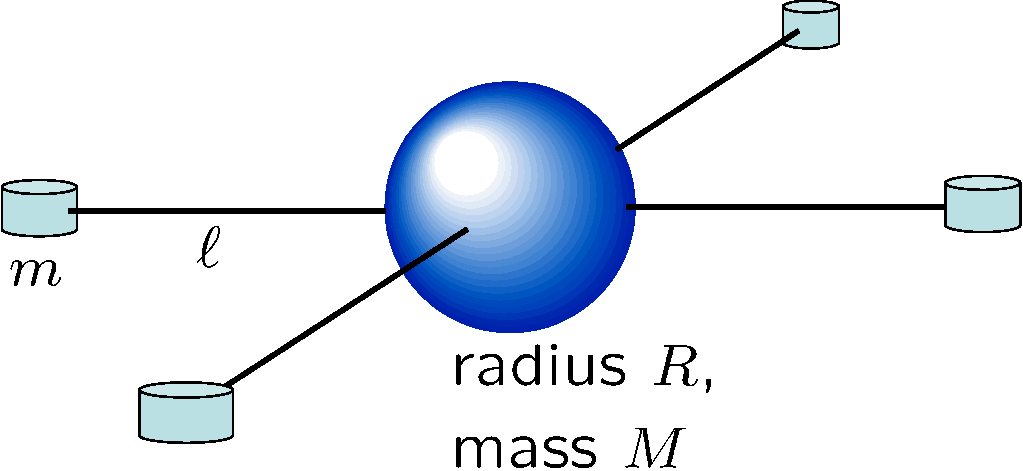
\includegraphics[width=0.6\textwidth]{chap3_multirotor/figures/quadrotor_inertia}\\
  \caption{The moments of inertia for the quadrotor are calculated
  assuming a spherical dense center with mass $M$ and radius $R$,
  and point masses of mass $m$ located at a distance of $\ell$ from
  the center.}%
  \label{fig:quadrotor_inertia}
\end{figure}
As shown in Figure~\ref{fig:quadrotor_inertia}, the quadrotor is
essentially symmetric about all three axes, therefore
$J_{xy}=J_{xz}=J_{yz}=0$ which implies that
\[
\mathbf{J} =
    \begin{pmatrix}
    J_{x}   & 0       & 0 \\
    0       & J_{y}   & 0 \\
    0 & 0       & J_{z}
    \end{pmatrix}.
\]
Therefore
\begin{align*}
\mathbf{J}^{-1}
    &= \begin{pmatrix}
        \frac{1}{J_x} & 0 & 0 \\
        0 & \frac{1}{J_y} & 0 \\
        0 & 0 & \frac{1}{J_z}
       \end{pmatrix}.
\end{align*}
The inertia for a solid sphere is given by
$J=2MR^2/5$\cite{HallidayResnick}.  Therefore
\begin{align*}
J_x &= \frac{2MR^2}{5} + 2\ell^2m \\
J_y &= \frac{2MR^2}{5} + 2\ell^2m \\
J_z &= \frac{2MR^2}{5} + 4\ell^2m.
\end{align*}


Defining $\mathbf{m}^b \defeq (\tau_{\phi}, \tau_{\theta},
\tau_{\psi})^T$ we can write Eq.~\eqref{eq:newton_rotation} in body
coordinates as
\begin{align*}
\begin{pmatrix} \dot{p} \\ \dot{q} \\ \dot{r} \end{pmatrix}
&= \begin{pmatrix}
        \frac{1}{J_x} & 0 & 0 \\
        0 & \frac{1}{J_y} & 0 \\
        0 & 0 & \frac{1}{J_z}
    \end{pmatrix}
    \left[
    \begin{pmatrix}
        0 & r & -q \\
        -r & 0 & p \\
        q & -p & 0
    \end{pmatrix}
    \begin{pmatrix}
    J_{x}   & 0       & 0 \\
    0       & J_{y}   & 0 \\
    0       & 0       & J_{z}
    \end{pmatrix}
    \begin{pmatrix} p \\ q \\ r \end{pmatrix}
    + \begin{pmatrix} \tau_{\phi} \\ \tau_{\theta} \\ \tau_{\psi} \end{pmatrix}
    \right] \\
&= \begin{pmatrix}
    \frac{J_y-J_z}{J_x} qr\\
    \frac{J_z-J_x}{J_y} pr\\
    \frac{J_x-J_y}{J_z} pq\\
    \end{pmatrix}
    + \begin{pmatrix}
    \frac{1}{J_x} \tau_{\phi} \\
    \frac{1}{J_y} \tau_{\theta} \\
    \frac{1}{J_z} \tau_{\psi}
    \end{pmatrix}.
\end{align*}


The six degree of freedom model for the quadrotor kinematics and
dynamics can be summarized as follows:
\begin{align}
\begin{pmatrix} \dot{p}_n \\ \dot{p}_e \\ \dot{h} \end{pmatrix}
&= \begin{pmatrix} c\theta c\psi & s\phi s\theta c\psi - c\phi s\psi
    & c\phi s\theta c\psi + s\phi s\psi \\
    c\theta s\psi &  s\phi s\theta s\psi + c\phi c\psi
    & c\phi s\theta s\psi - s\phi c\psi  \\
    s\theta & -s\phi c\theta & -c\phi c\theta
    \end{pmatrix}
    \begin{pmatrix} u \\ v \\ w \end{pmatrix}
    \label{eq:kin-eom-xyh} \\
\begin{pmatrix} \dot{u} \\ \dot{v} \\ \dot{w} \end{pmatrix}
&= \begin{pmatrix} rv-qw \\ pw-ru \\ qu-pv \end{pmatrix} +
    \frac{1}{m} \begin{pmatrix} f_x \\ f_y \\ f_z \end{pmatrix},
    \label{eq:kin-eom-v}\\
\begin{pmatrix} \dot{\phi} \\ \dot{\theta} \\ \dot{\psi} \end{pmatrix}
& = \begin{pmatrix}
    1 & \sin\phi\tan\theta & \cos\phi\tan\theta \\
    0 & \cos\phi & -\sin\phi \\
    0 & \frac{\sin\phi}{\cos\theta} & \frac{\cos\phi}{\cos\theta}
    \end{pmatrix}
    \begin{pmatrix} p \\ q \\ r \end{pmatrix}
    \label{eq:kin-eom-euler}\\
\begin{pmatrix} \dot{p} \\ \dot{q} \\ \dot{r} \end{pmatrix}
&= \begin{pmatrix}
    \frac{J_y-J_z}{J_x} qr\\
    \frac{J_z-J_x}{J_y} pr\\
    \frac{J_x-J_y}{J_z} pq\\
    \end{pmatrix}
    + \begin{pmatrix}
    \frac{1}{J_x} \tau_{\phi} \\
    \frac{1}{J_y} \tau_{\theta} \\
    \frac{1}{J_z} \tau_{\psi}
    \end{pmatrix}.
    \label{eq:kin-eom-omega}
\end{align}

%%%%%%%%%%%%%%%%%%%%%%%%%%%%%%%%%%%%%%%%%%%%%%%%%%%%%%%%%%%%%
\section{Forces and Moments} \label{chap:forces}
%%%%%%%%%%%%%%%%%%%%%%%%%%%%%%%%%%%%%%%%%%%%%%%%%%%%%%%%%%%%%

The objective of this section is to describe the forces and torques
that act on the quadrotor.  Since there are no aerodynamic lifting
surfaces, we will assume that the aerodynamic forces and moments are
negligible.

The forces and moments are primarily due to gravity and the four
propellers.

\begin{figure}[hhhhtb]
  % Requires \usepackage{graphicx}
  \centering
  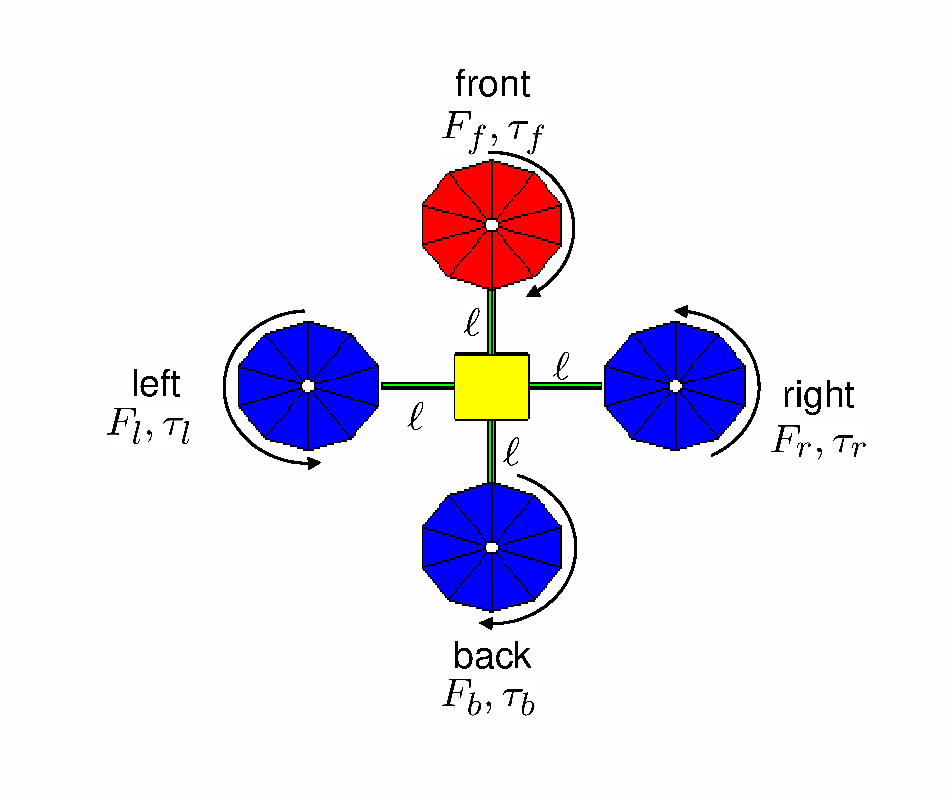
\includegraphics[width=0.6\textwidth]{chap3_multirotor/figures/quadrotor_top_view}\\
  \caption{The top view of the quadrotor.  Each motor produces an upward
  force $F$ and a torque $\tau$.  The front and back motors spin clockwise
  and the right and left motors spin counterclockwise.}%
  \label{fig:quadrotor_top_view}
\end{figure}


\begin{figure}[hhhhtb]
  % Requires \usepackage{graphicx}
  \centering
  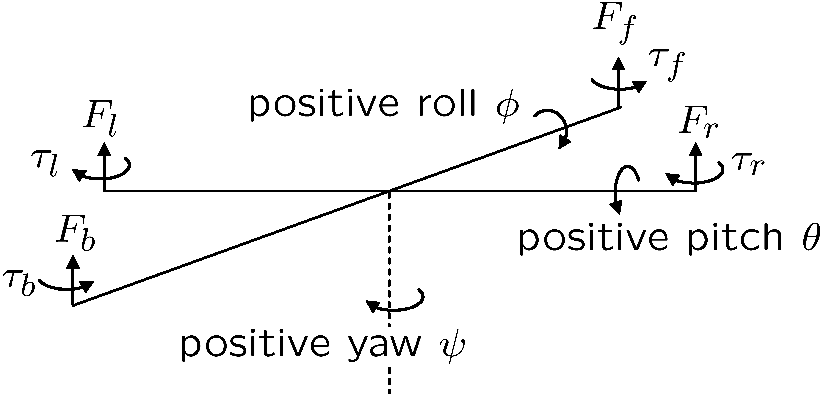
\includegraphics[width=0.6\textwidth]{chap3_multirotor/figures/quadrotor_define_angles}\\
  \caption{Definition of the forces and torques acting on the quadrotor.}%
  \label{fig:quadrotor_define_angles}
\end{figure}


Figure~\ref{fig:quadrotor_top_view} shows a top view of the
quadrotor systems.  As shown in
Figure~\ref{fig:quadrotor_define_angles}, each motor produces a
force $F$ and a torque $\tau$.  The total force acting on the
quadrotor is given by
\[
F = F_f + F_r + F_b + F_l.
\]
The rolling torque is produced by the forces of the right and left
motors as
\[
\tau_{\phi} = \ell(F_l - F_r).
\]
Similarly, the pitching torque is produced by the forces of the
front and back motors as
\[
\tau_{\theta} = \ell(F_f - F_b).
\]
Due to Newton's third law, the drag of the propellers produces a
yawing torque on the body of the quadrotor.  The direction of the
torque will be in the oppositive direction of the motion of the
propeller.  Therefore the total yawing torque is given by
\[
\tau_{\psi} = \tau_r + \tau_l - \tau_f - \tau_b.
\]

The lift and drag produced by the propellers is proportional to the
square of the angular velocity.  We will assume that the angular
velocity is directly proportional to the pulse width modulation
commend sent to the motor.  Therefore, the force and torque of each
motor can be expressed as
\begin{align*}
F_{\ast} &= k_1 \delta_{\ast} \\
\tau_{\ast} &= k_2 \delta_{\ast},
\end{align*}
where $k_1$ and $k_2$ are constants  that need to be determined
experimentally, $\delta_{\ast}$ is the motor command signal, and
$\ast$ represents $f$, $r$, $b$, and $l$.

Therefore, the forces and torques on the quadrotor can be written in
matrix form as
\[
\begin{pmatrix}
    F \\
    \tau_{\phi} \\
    \tau_{\theta} \\
    \tau_{\psi}
\end{pmatrix} =
\begin{pmatrix}
    k_1 & k_1 & k_1 & k_1 \\
    0 & -\ell k_1 & 0 & \ell k_1 \\
    \ell k_1 & 0 & -\ell k_1 & 0 \\
    -k_2 & k_2 & -k_2 & k_2
\end{pmatrix}
\begin{pmatrix}
    \delta_f \\
    \delta_r \\
    \delta_b \\
    \delta_l
\end{pmatrix}
\defeq \mathcal{M}
\begin{pmatrix}
    \delta_f \\
    \delta_r \\
    \delta_b \\
    \delta_l
\end{pmatrix}.
\]

The control strategies derived in subsequent sections will specify
forces and torques.  The actual motors commands can be found as
\[
\begin{pmatrix}
    \delta_f \\
    \delta_r \\
    \delta_b \\
    \delta_l
\end{pmatrix}
= \mathcal{M}^{-1}\emph{}
\begin{pmatrix}
    F \\
    \tau_{\phi} \\
    \tau_{\theta} \\
    \tau_{\psi}
\end{pmatrix}.
\]
Note that the pulse width modulation commands are required to be
between zero and one.


In addition to the force exerted by the motor, gravity also exerts a
force on the quadrotor.  In the vehicle frame $\mathcal{F}^v$, the
gravity force acting on the center of mass is given by
\[
\mathbf{f}_g^v = \begin{pmatrix} 0 \\ 0 \\ mg \end{pmatrix}.
\]
However, since $\mathbf{v}$ in Equation~\eqref{eq:kin-eom-v} is expressed
in $\mathcal{F}^b$, we must transform to the body frame to give
\begin{align*}
\mathbf{f}_g^b &= R_{v}^{b} \begin{pmatrix} 0 \\ 0 \\ mg \end{pmatrix} \\
&= \begin{pmatrix}
  -mg\sin\theta \\ mg\cos\theta\sin\phi \\ mg\cos\theta\cos\phi
  \end{pmatrix}.
\end{align*}

Therefore,
equations~\eqref{eq:kin-eom-xyh}--\eqref{eq:kin-eom-omega} become
\begin{align}
\begin{pmatrix} \dot{p}_n \\ \dot{p}_e \\ \dot{h} \end{pmatrix}
&= \begin{pmatrix} c\theta c\psi & s\phi s\theta c\psi - c\phi s\psi
    & c\phi s\theta c\psi + s\phi s\psi \\
    c\theta s\psi &  s\phi s\theta s\psi + c\phi c\psi
    & c\phi s\theta s\psi - s\phi c\psi  \\
    s\theta & -s\phi c\theta & -c\phi c\theta
    \end{pmatrix}
    \begin{pmatrix} u \\ v \\ w \end{pmatrix}
    \label{eq:kin-eom-xyh2} \\
\begin{pmatrix} \dot{u} \\ \dot{v} \\ \dot{w} \end{pmatrix}
&= \begin{pmatrix} rv-qw \\ pw-ru \\ qu-pv \end{pmatrix}
    + \begin{pmatrix}
  -g\sin\theta \\ g\cos\theta\sin\phi \\ g\cos\theta\cos\phi
  \end{pmatrix}+
    \frac{1}{m} \begin{pmatrix} 0 \\ 0 \\ -F \end{pmatrix},
    \label{eq:kin-eom-v2}\\
\begin{pmatrix} \dot{\phi} \\ \dot{\theta} \\ \dot{\psi} \end{pmatrix}
& = \begin{pmatrix}
    1 & \sin\phi\tan\theta & \cos\phi\tan\theta \\
    0 & \cos\phi & -\sin\phi \\
    0 & \frac{\sin\phi}{\cos\theta} & \frac{\cos\phi}{\cos\theta}
    \end{pmatrix}
    \begin{pmatrix} p \\ q \\ r \end{pmatrix},
    \label{eq:kin-eom-euler2}\\
\begin{pmatrix} \dot{p} \\ \dot{q} \\ \dot{r} \end{pmatrix}
&= \begin{pmatrix}
    \frac{J_y-J_z}{J_x} qr\\
    \frac{J_z-J_x}{J_y} pr\\
    \frac{J_x-J_y}{J_z} pq\\
    \end{pmatrix}
    + \begin{pmatrix}
    \frac{1}{J_x} \tau_{\phi} \\
    \frac{1}{J_y} \tau_{\theta} \\
    \frac{1}{J_z} \tau_{\psi}
    \end{pmatrix}.
    \label{eq:kin-eom-omega2}
\end{align}

%%%%%%%%%%%%%%%%%%%%%%%%%%%%%%%%%%%%%%%%%%%%%%%%%%%%%%%%%%%%%%%5
\section{Simplified Models}

Equations~\eqref{eq:kin-eom-xyh2}--\eqref{eq:kin-eom-omega2} are the
equations of motion to be used in our six degree-of-freedom
simulator.  However, they are not appropriate for control design for
several reasons. The first reason is that they are too complicated
to gain significant insight into the motion.  The second reason is
that the position and orientation are relative to the inertial world
fixed frame, whereas camera measurements will measure position and
orientation of the target with respect to the camera frame.

%----------------------------------------------------------------
\subsection{Model for estimation}
%----------------------------------------------------------------
For the quadrotor, we are not able to estimate the inertial position
or the heading angle $\psi$.  Rather, we will be interested in the
relative position and heading of the quadrotor with respect to a
ground target.  The relative position of the quadrotor will be
measured in the vehicle-1 frame, i.e., the vehicle frame after it
has been rotated by the heading vector $\psi$.  The vehicle-1 frame
is convenient since $x$, $y$, and $z$ positions are still measured
relative to a flat earth, but they are vehicle centered quantities
as opposed to inertial quantities.  Let $p_x$, $p_y$, and $p_z$
denote the relative position vector between the target and the
vehicle resolved in the $v1$ frame.  Therefore
Eq~\eqref{eq:kin-eom-xyh2} becomes
\begin{equation}     \label{eq:kin-eom-xyh3}
\begin{pmatrix} \dot{p}_x \\ \dot{p}_y \\ \dot{p}_z \end{pmatrix}
= \begin{pmatrix} c\theta & s\phi s\theta
    & c\phi s\theta \\
    0 &  c\phi
    & - s\phi  \\
    -s\theta & s\phi c\theta & c\phi c\theta
    \end{pmatrix}
    \begin{pmatrix} u \\ v \\ w \end{pmatrix}.
\end{equation}

%----------------------------------------------------------------
\subsection{Model for control design}
%----------------------------------------------------------------

Assuming that $\phi$ and $\theta$ are small,
Equation~\eqref{eq:kin-eom-euler2} can be simplified as
\begin{equation}\label{eq:kin-eom-euler3}
\begin{pmatrix} \dot{\phi} \\ \dot{\theta} \\ \dot{\psi} \end{pmatrix}
=  \begin{pmatrix} p \\ q \\ r \end{pmatrix}.
\end{equation}
Similarly, Equation~\eqref{eq:kin-eom-omega2} is simplified by
assuming that the Coriolis terms $qr$, $pr$, and $pq$, are small to
obtain
\begin{equation}\label{eq:kin-eom-omega3}
\begin{pmatrix} \dot{p} \\ \dot{q} \\ \dot{r} \end{pmatrix}
=   \begin{pmatrix}
    \frac{1}{J_x} \tau_{\phi} \\
    \frac{1}{J_y} \tau_{\theta} \\
    \frac{1}{J_z} \tau_{\psi}
    \end{pmatrix}.
\end{equation}
Combining Eq.~\eqref{eq:kin-eom-euler3}
and~\eqref{eq:kin-eom-omega3} we get
\begin{equation}\label{eq:kin-euler-ddot}
\begin{pmatrix} \ddot{\phi} \\ \ddot{\theta} \\ \ddot{\psi} \end{pmatrix}
=  \begin{pmatrix}
    \frac{1}{J_x} \tau_{\phi} \\
    \frac{1}{J_y} \tau_{\theta} \\
    \frac{1}{J_z} \tau_{\psi}
    \end{pmatrix}.
\end{equation}

Differentiating Eq.~\eqref{eq:kin-eom-xyh2} and neglecting
$\dot{R}_b^v$ gives
\begin{equation}\label{eq:kin-eom-xyh4}
\begin{pmatrix} \ddot{p}_n \\ \ddot{p}_e \\ \ddot{p}_d \end{pmatrix}
= \begin{pmatrix} c\theta c\psi & s\phi s\theta c\psi - c\phi s\psi
    & c\phi s\theta c\psi + s\phi s\psi \\
    c\theta s\psi &  s\phi s\theta s\psi + c\phi c\psi
    & c\phi s\theta s\psi - s\phi c\psi  \\
    -s\theta & s\phi c\theta & c\phi c\theta
    \end{pmatrix}
    \begin{pmatrix} \dot{u} \\ \dot{v} \\ \dot{w} \end{pmatrix}.
\end{equation}
Neglecting the Coriolis terms and plugging Eq.~\eqref{eq:kin-eom-v2}
into Eq.~\eqref{eq:kin-eom-xyh4} and simplifying gives
\begin{equation}\label{eq:kin-xyh-ddot}
\begin{pmatrix} \ddot{p}_n \\ \ddot{p}_e \\ \ddot{p}_d \end{pmatrix}
= \begin{pmatrix} 0 \\ 0 \\ g \end{pmatrix} +
\begin{pmatrix}
    -c\phi s\theta c\psi - s\phi s\psi \\
    -c\phi s\theta s\psi + s\phi c\psi  \\
    -c\phi c\theta
    \end{pmatrix}
    \frac{F}{m}.
\end{equation}

Therefore, the simplified inertial model is given by
\begin{align}
\ddot{p}_n    &= \left(-\cos\phi \sin\theta \cos\psi - \sin\phi
\sin\psi \right) \frac{F}{m}
\label{eq:quadrotor-simple-pn} \\
\ddot{p}_e    &= \left( -\cos\phi \sin\theta \sin\psi + \sin\phi
\cos\psi \right) \frac{F}{m}
\label{eq:quadrotor-simple-pe} \\
\ddot{p}_d      &= g - \left( \cos\phi \cos\theta \right)
\frac{F}{m}
\label{eq:quadrotor-simple-h} \\
\ddot{\phi}   &= \frac{1}{J_x} \tau_{\phi}
\label{eq:quadrotor-simple-phi} \\
\ddot{\theta} &= \frac{1}{J_y} \tau_{\theta}
\label{eq:quadrotor-simple-theta} \\
\ddot{\psi}   &= \frac{1}{J_z} \tau_{\psi}.
\label{eq:quadrotor-simple-psi} \\
\end{align}

The dynamics given in
Equations~\eqref{eq:quadrotor-simple-pn}--\eqref{eq:quadrotor-simple-psi}
are expressed in the inertial frame.  This is necessary for the
simulator.  However, we will be controlling position, altitude, and
heading using camera frame measurements of a target position.  In
this setting heading is irrelevant.  Therefore, instead of
expressing the translational dynamics in the inertial frame, we will
express them in the vehicle-1 frame $\mathcal{F}^{v1}$, which is
equivalent to the inertial frame after rotating by the heading
angle.

Differentiating Eq.~\eqref{eq:kin-eom-xyh3} and neglecting
$\dot{R}_b^{v1}$ gives
\begin{equation}\label{eq:kin-eom-xyh5}
\begin{pmatrix} \ddot{p}_x \\ \ddot{p}_y \\ \ddot{p}_z \end{pmatrix}
= \begin{pmatrix} c\theta & s\phi s\theta
    & c\phi s\theta \\
    0 &  c\phi
    & - s\phi  \\
    -s\theta & s\phi c\theta & c\phi c\theta
    \end{pmatrix}
    \begin{pmatrix} \dot{u} \\ \dot{v} \\ \dot{w} \end{pmatrix}.
\end{equation}
Neglecting the Coriolis terms and plugging Eq.~\eqref{eq:kin-eom-v2}
into Eq.~\eqref{eq:kin-eom-xyh5} and simplifying gives
\begin{equation}\label{eq:kin-xyh-ddot}
\begin{pmatrix} \ddot{p}_x \\ \ddot{p}_y \\ \ddot{p}_z \end{pmatrix}
= \begin{pmatrix} 0 \\ 0 \\ g \end{pmatrix} +
\begin{pmatrix}
    -c\phi s\theta \\
    s\phi \\
    -c\phi c\theta
    \end{pmatrix}
    \frac{F}{m}.
\end{equation}

Therefore, the simplified model in the vehicle-1 frame is given by
\begin{align}
\ddot{p}_x    &= -\cos\phi \sin\theta \frac{F}{m}
\label{eq:quadrotor-simple-px} \\
\ddot{p}_y    &= \sin\phi \frac{F}{m}
\label{eq:quadrotor-simple-py} \\
\ddot{p}_z    &= g - \cos\phi \cos\theta \frac{F}{m}
\label{eq:quadrotor-simple-pz} \\
\ddot{\phi}   &= \frac{1}{J_x} \tau_{\phi}
\label{eq:quadrotor-simple-phi2} \\
\ddot{\theta} &= \frac{1}{J_y} \tau_{\theta}
\label{eq:quadrotor-simple-theta2} \\
\ddot{\psi}   &= \frac{1}{J_z} \tau_{\psi}.
\label{eq:quadrotor-simple-psi2} \\
\end{align}

} 
%%%%%%%%%%%%%%%%%% End BIG omit

\section{Multirotor Aerial Vehicles, Mahony, Kumar, Corke, IEEE RA Mag, Sept, 2020.}
The model in this paper is nicely done.

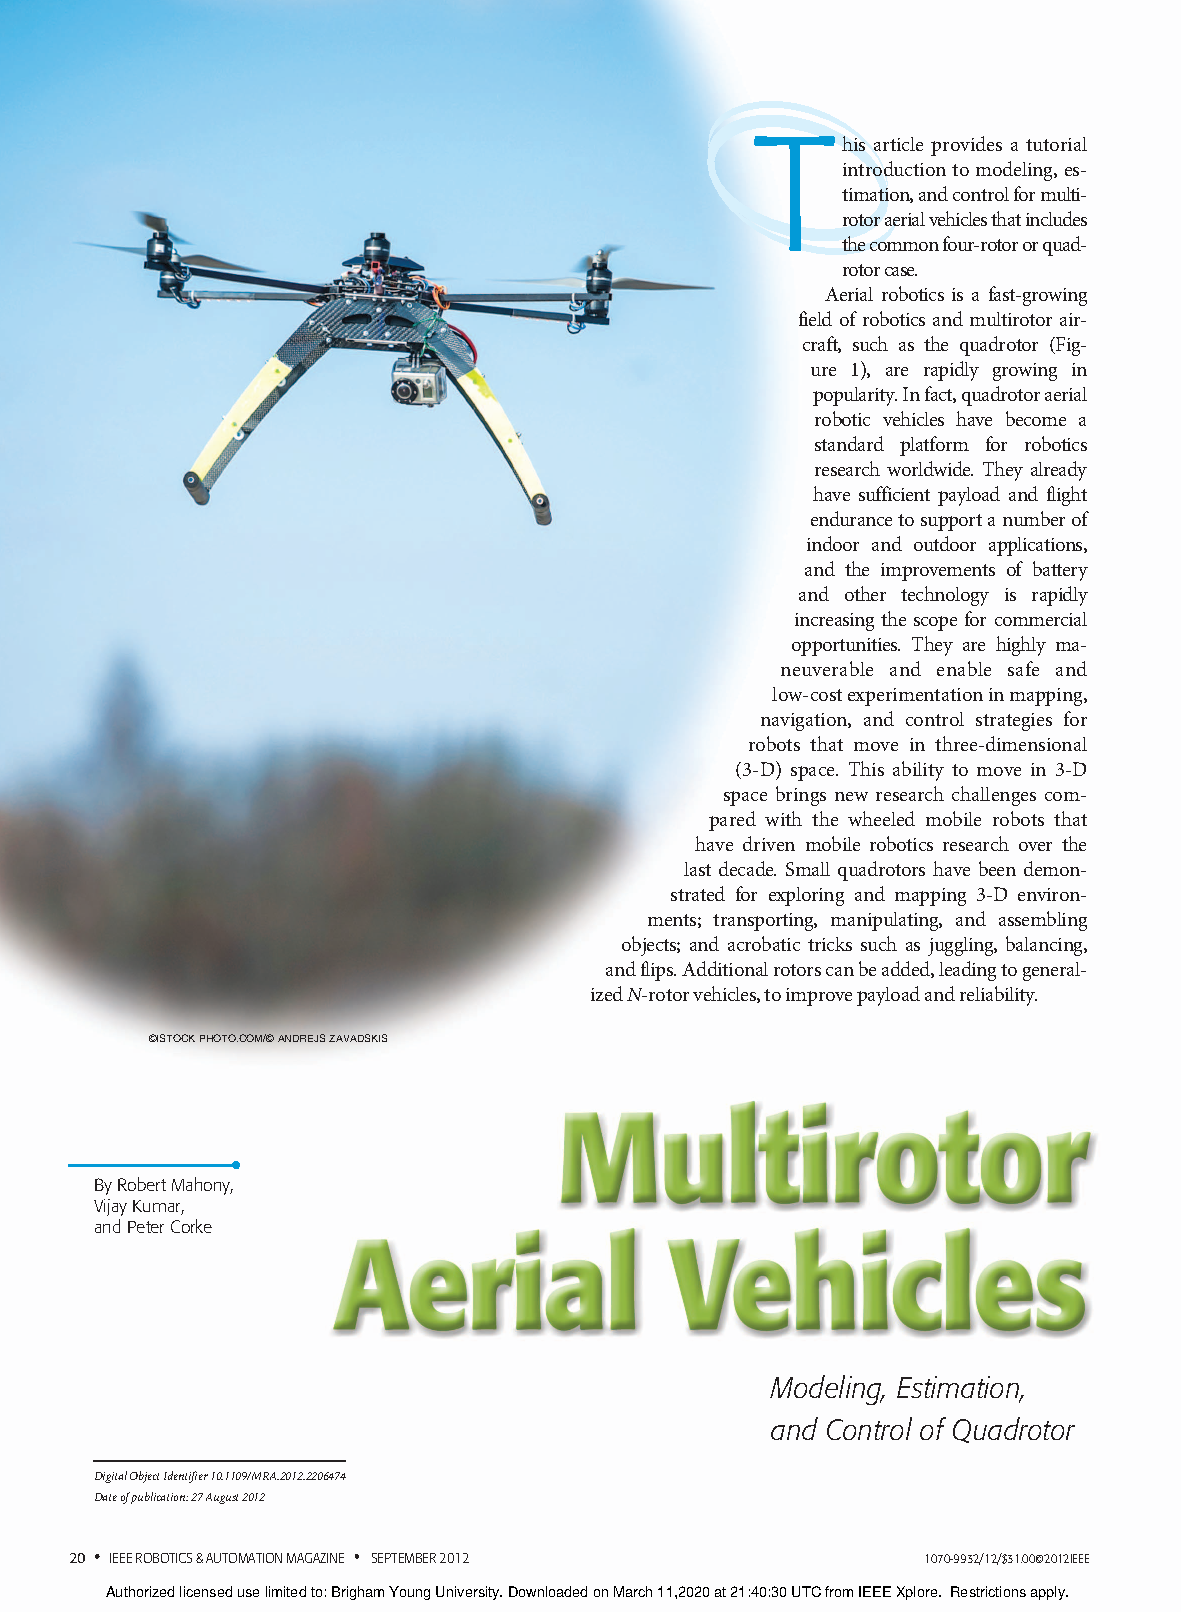
\includepdf[pages=-,scale=.8,pagecommand={}]{chap3_multirotor/papers/MahonyKumarCorke.pdf}




